\chapter{Design Automation}\label{ch:designautomate}
\openepigraph{%
    Nicht Kunst und Wissenschaft allein,\\Geduld will bei dem Werke sein.%\\[0.25\baselineskip]
    %Not Art and Science serve alone;\\Patience must in the work be shown
}{Johann Wolfgang von Goethe}
\openepigraph{During human progress, every science is evolved out of its corresponding art.}{Herbert Spencer}
\section{Truth Table Generation}
After the network has been trained, we need to generate the truth table for every neuron. Currently, we support a $generateTruthTable$ method with the class, to allow the user to generate truth tables for only specific layers for inspection. In practice this is specially useful, as the model size increase. \\
The truth table for a neuron with a fan-in of 6 bits requires $2^{6} = 64$ entries. However, in complicated data-sets it is impractical to keep the fan-in at only 6 bits. If we increase the number of bits for the fan-in of each neuron, the number of entries grow exponentially. For instance if the neuron has 20 input bits, it will have $2^{20} = 1048576$ entries. Clearly, for such models we not only need to allow on the go calculation of the truth table for each layer, but also the truth table for each neuron. This will allow us to extract more parallelism out of the process. Support for per-neuron calculation of truth tables will be added soon.
\newthoughtpar{Structure of Truth Table}
We can see in Listing \ref{layerttablestruct}, the structure of the truth table of a model which has 3 neurons fan-in of 3, with a bit-width of 1. The keys are the neuron IDs of the layer (in this case linear1). Once the key is accessed, we get a list of lists, the first list containing the binary input to a neuron, and the second containing the output for that specific input. While the first list does not have any utility as the input bits are inumerated in a fixed fashion, we will keep this functionality for now.

\begin{lstlisting}[language=Python, caption=Structure of the Truth Table for a layer, label=layerttablestruct]
>>> print(model.linear1.truthtable)
OrderedDict([('0',
              [['000', '001', '010', '011', '100', '101', '110', '111'],
               ['1', '1', '1', '0', '1', '0', '0', '0']]),
             ('1',
              [['000', '001', '010', '011', '100', '101', '110', '111'],
               ['1', '0', '1', '0', '1', '0', '1', '0']]),
             ('2',
              [['000', '001', '010', '011', '100', '101', '110', '111'],
               ['1', '0', '1', '0', '1', '0', '1', '0']])])
\end{lstlisting}

\newpage



\marginpar{\centering
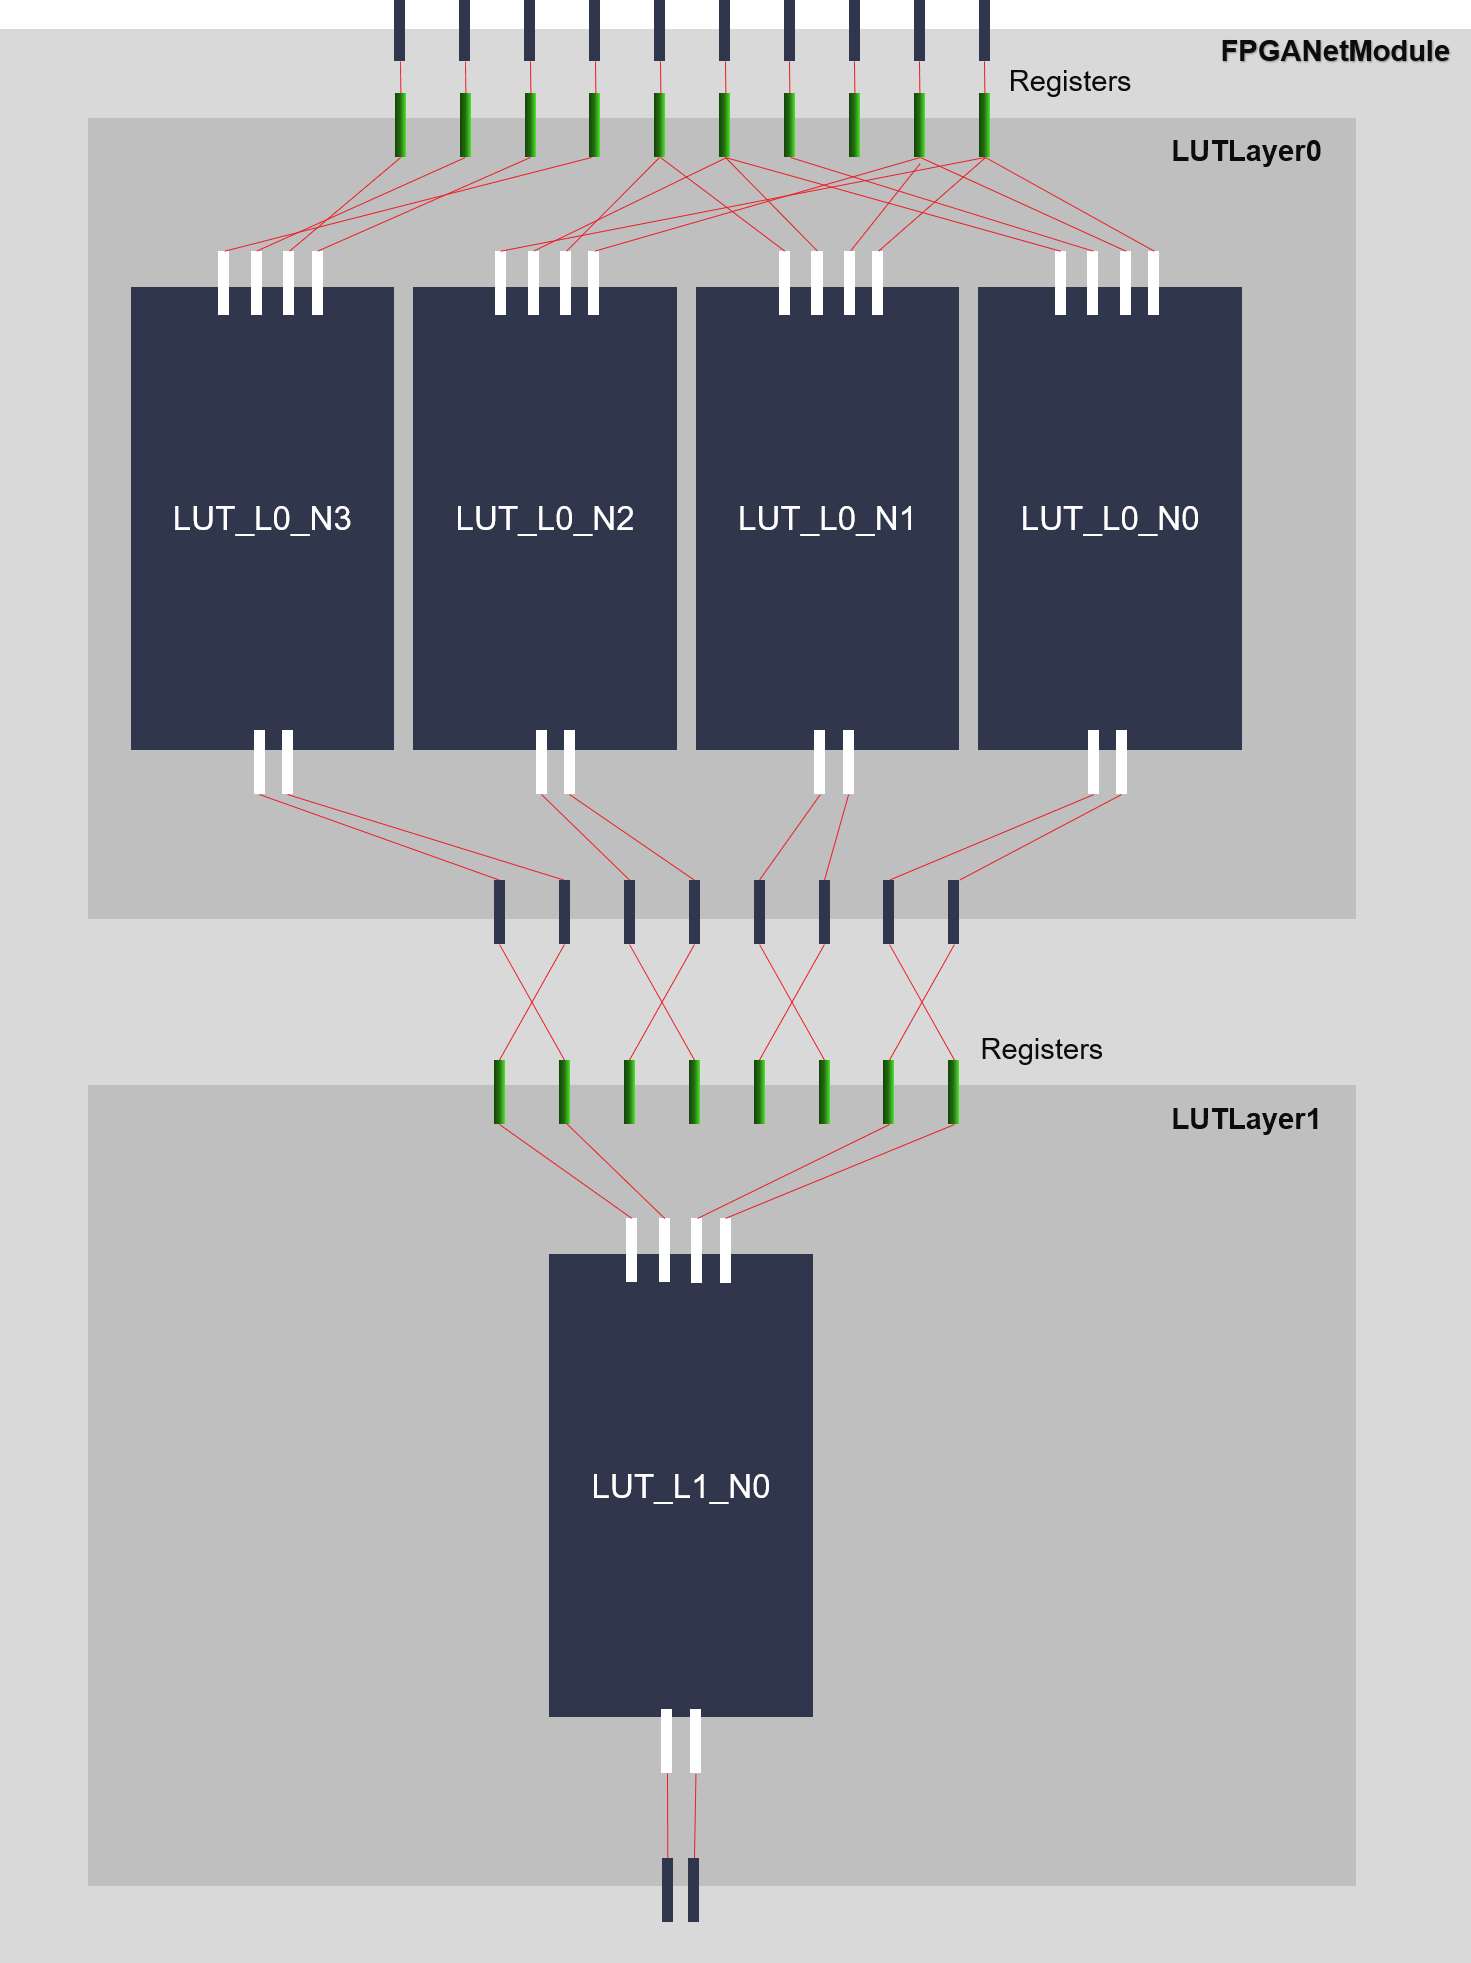
\includegraphics[width=500pt]{figures/bison/fpganetmodule.png}
\captionof{figure}{VERILOG Code Generation Sub-Modules.}
\label{fig:fpganetmodule}
% \endgroup
}   

\newpage
% \begin{figure}[h]
%     \centering
%     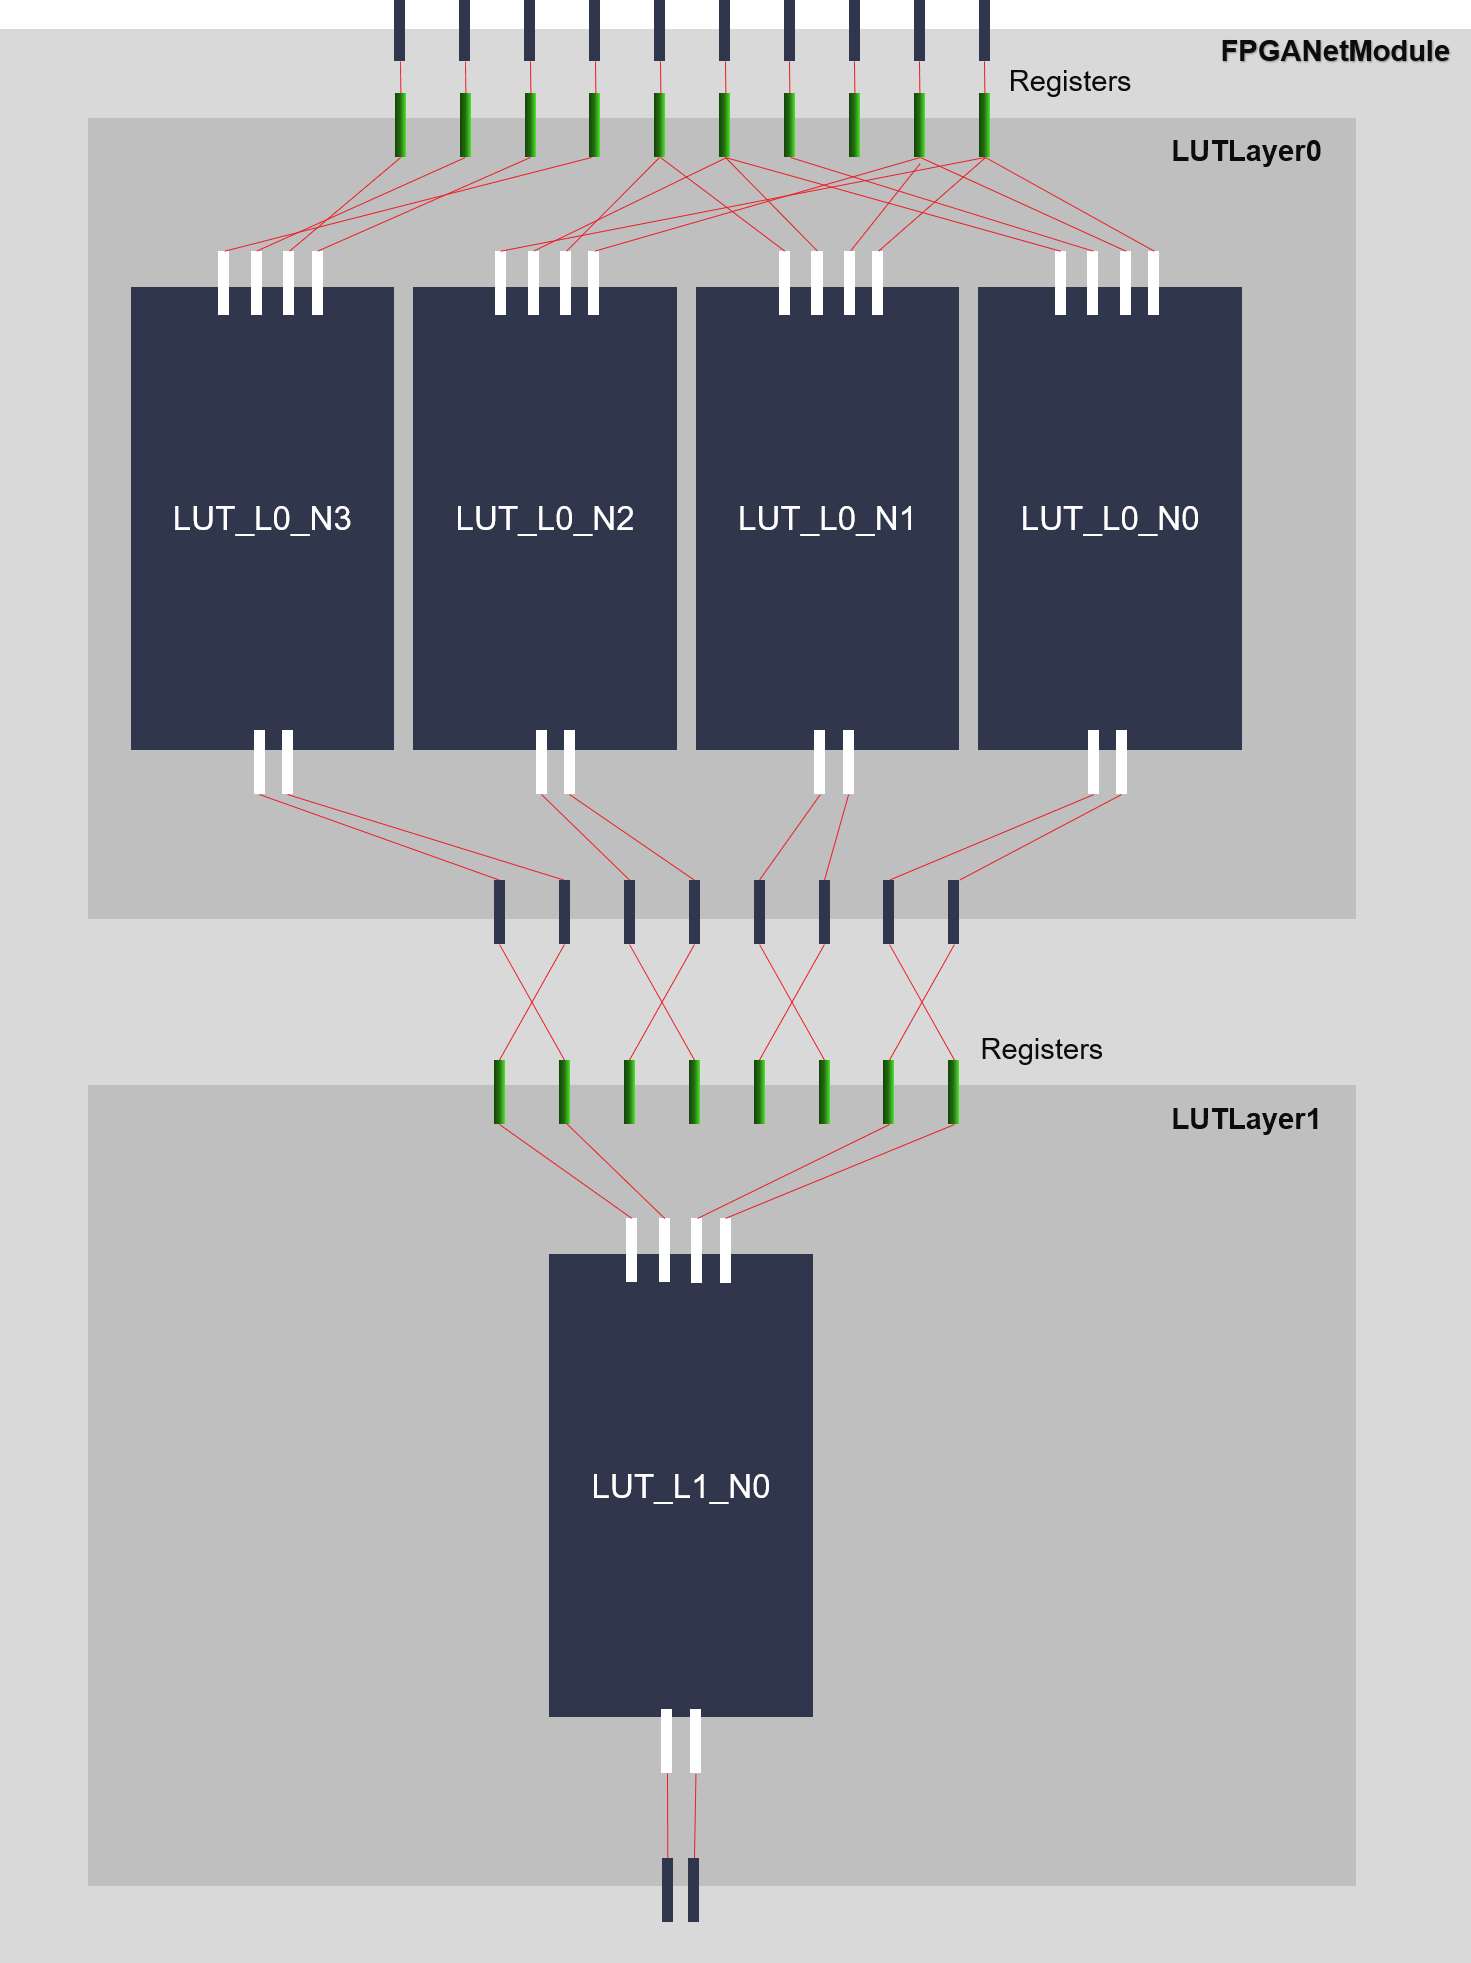
\includegraphics[width=330pt]{figures/bison/fpganetmodule.png}
%     \caption{VERILOG Code Generation Structure}
%     \label{fig:fpganetmodule}
% \end{figure}
 
\begin{table}
    \begin{sidecaption}[Size and Time estimates for VERILOG Generation]{% 
        Rough estimates of the file size to store the truth table for 1 neuron with a specific fan-in in bits, and the time it takes to write the '.v' file.
    }[designautomate:tab:filesize]
\begin{threeparttable}
\begin{tabular}{lrr}
\hline
Bits & File Size(MB) & Time (seconds) \\ \hline
15   & 0.85          & 56      \\
16   & 1.8           & 119     \\
18   & 6.9           & 502     \\
20   & 29.0          & 2022    \\ \hline
\end{tabular}
\end{threeparttable}
\end{sidecaption}
\end{table}

\section{VERILOG Code Generation}

The VERILOG generator has been integrated as a VerilogGenerator class. This class takes in a model, identifies all the layers that are 'SparseLinear'. While Truth Table Generation is supported for all topologies (Linear and Convolution), we do not currently support VERILOG Code Generation for 'DenseQuantLinear' and 'SparseConv'. The SparseConv implementation will need a lot of thought, as it needs to incorporate any form of folding that may be necessary. VERILOG Generator for a Fully-Unfolded SparseConv will be integrated into the library at a later time.\\
From the code sample below, it becomes evident that we do not use any LUT primitives when generating the VERILOG code for the network. We instead define the entire truth table, and leave it up to the Logic Synthesis tool to generate the optimal 'hardware building block'. It is a very interesting research question, to explore whether a more optimal solution is discovered by the synthesis tool or does it have any benefit to define primitives ourselves. 
Further, due to the nature of how the verilog code itself is generated, the 'file size' and the time to generate the truth table explodes exponentially as well (\cref{designautomate:tab:filesize}). While the current VERILOG generator is purely sequential, we hope to extend functionality to generate the codes in a more parallel fashion. This would allow us to test a wider array of topologies faster. 


\newthoughtpar{VERILOG code sample}
We attach a code sample for VERILOG code generated for the Neural Network in the previos section (Single Layer, 3 Neurons with each neuron having a fan in of 3 bits). Note that this code sample is for synthesis of a \textbf{purely combinational circuit}, no registers have been placed at the input or output. This library supports VERILOG code generation with intermediate registers, and will be discussed later. \cref{fig:fpganetmodule} clearly shows how registers are implemented at the input and the intermediate layer.

\begin{lstlisting}[language=Verilog, caption=LogicNetModule.v, label=LogicNetModulev]
module LogicNetModule (input [4:0] M0, output[2:0] M1);
        LUTLayer0  LUTLayer0_inst (.M0(M0), .M1(M1));
endmodule
\end{lstlisting}

\begin{lstlisting}[language=Verilog, caption=LUTLayer0.v, label=LUTLayer0v]
module LUTLayer0 (input [4:0] M0, output [2:0] M1
);
wire [2:0] inpWire0_0 = {M0[0], M0[2], M0[4]};
LUT_L0_N0 LUT_L0_N0_inst (.M0(inpWire0_0), .M1(M1[0:0]));

wire [2:0] inpWire0_1 = {M0[1], M0[2], M0[3]};
LUT_L0_N1 LUT_L0_N1_inst (.M0(inpWire0_1), .M1(M1[1:1]));

wire [2:0] inpWire0_2 = {M0[0], M0[1], M0[2]};
LUT_L0_N2 LUT_L0_N2_inst (.M0(inpWire0_2), .M1(M1[2:2]));

endmodule
\end{lstlisting}

\begin{lstlisting}[language=Verilog, caption=LUTL0N0.v, label=LUTL0N0v]
module LUT_L0_N0 ( input [2:0] M0, output [0:0] M1 );
        reg [0:0] M1;
        always @ (M0) begin
                case (M0)
                        3'd0: M1 = 1'b1;
                        3'd1: M1 = 1'b1;
                        3'd2: M1 = 1'b1;
                        3'd3: M1 = 1'b0;
                        3'd4: M1 = 1'b1;
                        3'd5: M1 = 1'b0;
                        3'd6: M1 = 1'b0;
                        3'd7: M1 = 1'b0;
                endcase
        end
endmodule
\end{lstlisting}

\begin{lstlisting}[language=Verilog, caption=LUTL0N1.v, label=LUTL0N1v]
module LUT_L0_N1 ( input [2:0] M0, output [0:0] M1 );
        reg [0:0] M1;
        always @ (M0) begin
                case (M0)
                        3'd0: M1 = 1'b1;
                        3'd1: M1 = 1'b0;
                        3'd2: M1 = 1'b1;
                        3'd3: M1 = 1'b0;
                        3'd4: M1 = 1'b1;
                        3'd5: M1 = 1'b0;
                        3'd6: M1 = 1'b1;
                        3'd7: M1 = 1'b0;
                endcase
        end
endmodule
\end{lstlisting}

\begin{lstlisting}[language=Verilog, caption=LUTL0N2.v, label=LUTL0N2v]
module LUT_L0_N2 ( input [2:0] M0, output [0:0] M1 );
        reg [0:0] M1;
        always @ (M0) begin
                case (M0)
                        3'd0: M1 = 1'b1;
                        3'd1: M1 = 1'b0;
                        3'd2: M1 = 1'b1;
                        3'd3: M1 = 1'b0;
                        3'd4: M1 = 1'b1;
                        3'd5: M1 = 1'b0;
                        3'd6: M1 = 1'b1;
                        3'd7: M1 = 1'b0;
                endcase
        end
endmodule
\end{lstlisting}

\newpage


\begin{table}
    \begin{sidecaption}[Analytical vs.\ True LUT cost.]{%
        Comparing the Analytical LUT Cost formula with the results we actually get from synthesis of the network. Note that this is for a \textbf{purely combinational circuit} implementation of the Neural Network. 
    }[designautomate:tab:truelutcost]
\begin{threeparttable}
\begin{tabular}{lrr}
\hline
Analytical LUT cost & LUTs After Synthesis & Reduction     \\ \hline
128      & 80                & 1.6 $\times$  \\
272517   & 54336             & 5.01$\times$  \\
726180   & 76336             &  9.5$\times$  \\ \hline
% 11621540 & -                 &    -$\times$  \\ 
\end{tabular}
\end{threeparttable}
\end{sidecaption}
\end{table}


\begin{table}
\begin{threeparttable}
\begin{tabular}{llllrrrrr}
\hline
\multicolumn{3}{c}{Model}      & Analytical LUTs & \multicolumn{5}{c}{Resources}    \\ \hline
X  & BW & HL                   &                 & LUT   & FF   & DSP & BRAM & WNS  \\ \hline
3  & 2  & 64, 32, 32           & 266             & 132   & 160  & 0   & 0    & 4.04 \\
5  & 2  & 64, 32, 32           & 5586            & 2132  & 393  & 0   & 0    & 2.54 \\
3  & 4  & 64, 32, 32           & 45220           & 7117  & 3394 & 0   & 5    & 1.073\\
7  & 2  & 64, 32, 32           & 90706           & 22146 & 1533 & 0   & 0    & 1.073\\
4  & 3  & 64, 32, 32, 32, 32   & 50235           & 16338 & 1329 & 0   & 5    & 1.44 \\ \hline
\end{tabular}
\end{threeparttable}
\begin{caption}[Model Resource Costs]{%
    Analyzing the result of synthesizing neural networks trained on the Jet Substructure Classification problem by FPGA4HEP, using different Neuron Fan-Ins. The synthesized networks have registers between layers and at the input. Note that the clock target was 5ns. 
}
\label{designautomate:tab:fpga4hepwithregs}
\end{caption}
\end{table}
% & AUC-ROC
% & 85.28  
% & 87.48  
% & 89.46  
% & 86.78  
% & 88.8   

\section{Logic Synthesis and Analytical LUT estimates}
Logic synthesis is a key stage in the computer aided design flow of a FPGA. It is composed of a series of optimizations to improve the performance of the design. To support logic synthesis, our tool-flow is fairly straight forward. Once the VERILOG Generator has generated all the codes for each neuron, we can simply import the $synthesize\_and\_get\_resource\_counts$ function from $fpganet.synthesis$. Once called, it returns a list of all the hardware resource that are needed. It also generates a log file which contains a verbose description of the synthesized model. 

Upon synthesizing a few neural networks on Vivado using the Logic Synthesis tool-flow, we observed that the Analytical LUT cost was an overestimation. This can be seen in \cref{designautomate:tab:truelutcost}. In general, we observed that our Logic Synthesis tool optimized the implementation such that we only need a fraction of the actual estimate. This raises very interesting question about the topologies we can explore. We had restricted ourselves in topology exploration due to certain fan-ins being beyond the scope of fitting on any FPGA fabric. \\
The networks we have reported in later sections are all using our Analytical LUT Cost model, which is actually an overestimation as is evidenced by \cref{designautomate:tab:truelutcost}. It seems that as the Analytical LUT cost increases, the reduction in the true LUT resource needed is more notable, thought this claim needs a lot more testing to be proven empirically. \\
This LUT costs presented in \cref{designautomate:tab:truelutcost} only present purely combinational implementation of the neural network. After observing the cost of such an implementation, we need to look at the how the resource cost behaves when we have registers at intermediate stages (between layers). We also need to conduct some timing analysis of the circuit generated by this process.

\subsection{Resource cost with and without Registers in circuit}
As we see in \cref{fig:fpganetmodule}, between every LUTLayer the activations are wired to intermediate registers, this is also true for the input of the LogicNetModule. In this section we previously looked at the LUT cost reduction after synthesis without any registers (a purely combinational circuit). The LUT cost reduction for a network without registers between intermediate layers could be greater, due to the fact that now the optimization problem does not have a hierarchy (across layers). This could also cause an increase in the synthesis time. We observed a noticeable decrease in synthesis time for a circuit with registers, but do not provide empirical evidence to back this observation. 


\section{Timing Analysis}
In order to do some timing analysis on a basic LogicNet topology, we synthesized a small network by creating a fully-pipelined VERILOG description. After running synthesis, placement and Routing using Vivado, we observed a resource usage of 150 LUTs (from the analytical cost of 212 LUTs), and a minimum clock period of $0.768$~ns (frequency of 1.3~GHz), due to a very small circuit size. This indicates that there is potential for further reduction of resource footprint using logic minimization. Also note that the maximum clock frequency supported by the global clock network on the FPGA tested is 666 MHz, which leaves a large amount of slack for larger topologies. This actually stands true for more complicated topologies that we tested. These topologies are listed in \cref{designautomate:tab:fpga4hepwithregs}, the WNS stands for the 'Worst Negative Slack'. Slack is defined as the difference between the actual and the desired time for a timing path. A good FPGA design should have zero slack, if we have negative slack then the timing constraints we have specific for our design is not met. In such a scenario we can either relax our constraints or come up with a better design to meet these timing constraints we had initially specified. All the reported synthesis experiments in \cref{designautomate:tab:fpga4hepwithregs} are with a clock target of 5ns. For the first model in the table, this results in a frequency of $\frac{1000}{5-WNS} \approx 1042 MHz$. While it is evident that the frequency decreases as the LUT cost increases, we will also be conducting experiments with a more strict 1ns clock target in the future as well as more in-depth analysis of the LUT cost with and without registers.\\

It is also very interesting to note that in larger topologies, the logic synthesizer not only uses the LUTs, but also stores some neurons in the BRAMs. As we had stored truth tables themselves as primitives, it is really interesting to see what 'Hardware Building Blocks' are generated to store the Neurons. While this is interesting, as we make the clock target more strict, the synthesizer may choose to purely use LUTs. This is yet to be observed and more testing needs to be done to understand how the analytical LUTs differ from the true resource allocation of the synthesizer. \\


\clearpage

\clearpage
\section{Research Recess II – Synthesis}

The implications of \cref{designautomate:tab:truelutcost} to topology design is of great importance. We believe that there are two important questions we need to answer.
\subsection{Can we design a heuristic that aids LUT cost reduction for a neuron?}
In this library, we train neurons with static random connectivity. While this idea leads to sub-optimal accuracy, we are not too concerned with this as we can adopt any pruning technique and convert that into a mask-weight tensor and port that to a LogicNet model. An interesting question to ask is, is there a way to train each \textit{neuron}, such that during synthesis the LUT cost is dramatically lower than the analytical LUT cost? \\
This question is unanswered in this thesis. However, in this section, we hope to delve into this to some extent and define a way we can incorporate this into the training procedure. Our LogicNet library supports truth table calculation. This can be a slow process, but if a model only has to be deployed for inference; we can propose a training scheme that does take this into account. \\

PyEDA is a python library for Electronic Design Automation. Logic minimization is known to be a NP-Complete problem. It supports Truth Table Minimization. Instead of minimizing expressions, we can use our Truth Table Generator and integrate that with PyEDA to get the minimized truth table. It is important to note that this will significantly increase the train time of the neural network. Thus, we keep it beyond the scope of this thesis. We still however, nudge the idea of creating a cost function which takes the truth table minimization into account. Studying the hyper-parameter setting for such a cost function and its effect on the accuracy would be a very interesting topic. 

\subsection{Can we integrate congestion estimation in an FPGA with neural architecture search for non-layered topologies?}
There has been a lot of interest around congestion estimation for FPGAs. In a non-layered scenario, it could be really important to take congestion of an FPGA into account. The most efficient methods are based on fast-to-compute heuristics \cite{Swartz:1998:FRR:275107.275134} but they often have poor estimates. \cite{Yeager2007CongestionEA} uses a global router during placement, which gives more accurate congestion estimates, but at the cost of runtime. \\
The aforementioned methods provide estimates during place-and-route. Above a certain complexity of topology design, we may need to develop a heuristic which allows us to give a congestion estimate for a certain topology. This is a very complicated research problem, but there has been some progress in this direction. \cite{Samajdar2019ScalingTC} design directly in RTL component-level instantiations of DSP, BRAMs and URAMs and associated controller's for orchestrating data movement and manually leverage dedicated cascade interconnects for high frequency, nearest-neighbour data movement. \\
Given a netlist representation of a circuit, the elementary objective of congestion minimization is to minimize the total sum of wirelength for each net. Perhaps, it may also be a better endeavor to integrate certain design principles into topology constraints instead of attempting to get a real congestion estimation. This remains in our opinion an interesting research problem. It is a hard problem to formalize, and may be very interesting to implement. 